\section{Torque Measurement}

The previous version of the robot used a velocity-based control approach, setting a target velocity for the controller.
The new version of the robot features servo motors capable of current measurement and current control, which can be used to indirectly measure the torque applied to the motors.
Several experiments were conducted to understand the relationship between the measured current and the actual torque, detailed in the following sections.

\subsection{Experiment setup}
The experiment setup consists of a servo motor with a wheel attached as seen in \autoref{fig:torque_experiment_setup}.
The motor is securely mounted on the base plate, which in turn is clamped to a table.
A second table of the same height is placed opposite the wheel and on it rests the foot which holds up the free end of the axis.

\begin{figure}[htbp]
    \centering
    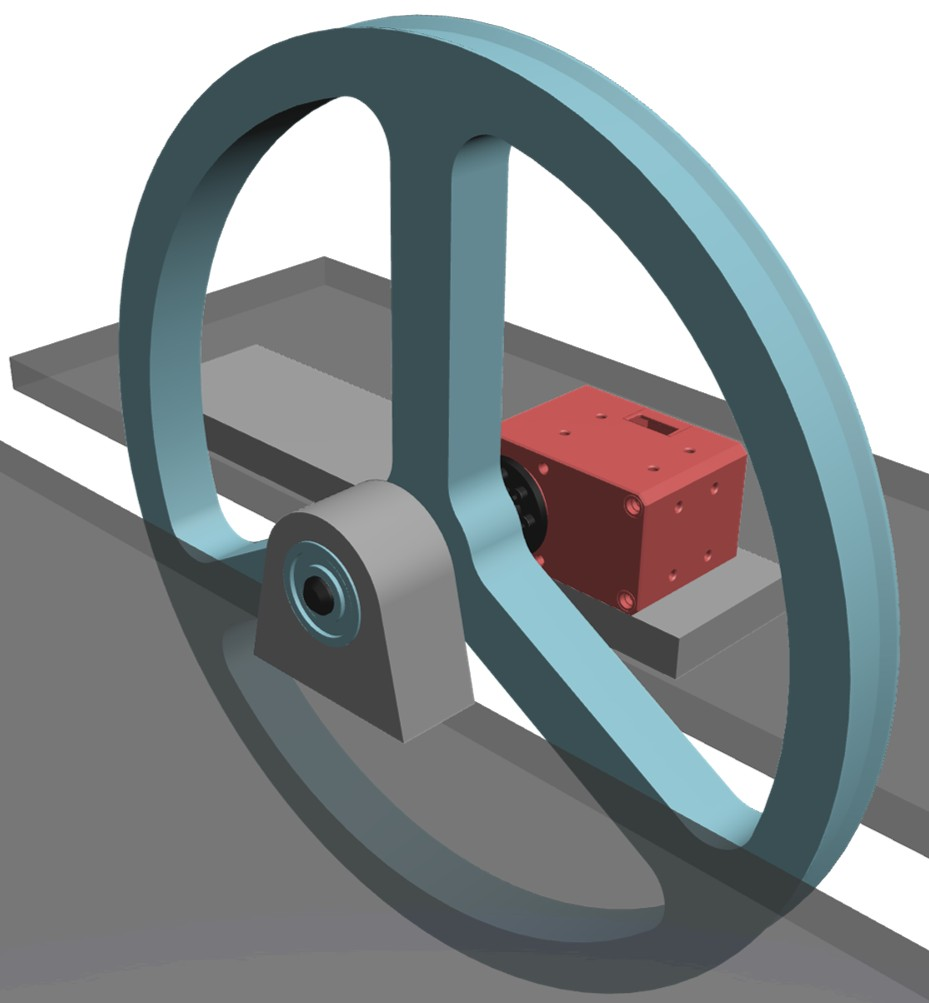
\includegraphics[width=0.8\linewidth]{images/torque_experiment_setup.jpg}
    \caption{Experiment setup for measuring torque.}
    \label{fig:torque_experiment_setup}
\end{figure}

The wheel pulls a set weight by a string, therefore applying a constant torque to the motor.
Depending on the direction in which the string is wrapped around the wheel, the applied torque can be either clockwise or anticlockwise.
The current is then measured while the weight is being moved up and down, both for clockwise and for anticlockwise torque.

\subsection{First Measurements}
For the first experiments, a metal weight of 1.056 kg was used, which applies a torque of 1.036 Nm to the motor. The motor is controlled using the internal velocity control,
which is the same control method used in the previous software version of the robot.
As a first experiment, the motor was simply moved upwards and downwards with the weight attached, holding the weight at the topmost position for 10 seconds.
The experiment has been repeated 4 times and the results can be seen in \autoref{fig:first_measurements}.
\begin{figure}[htbp]
    \centering
    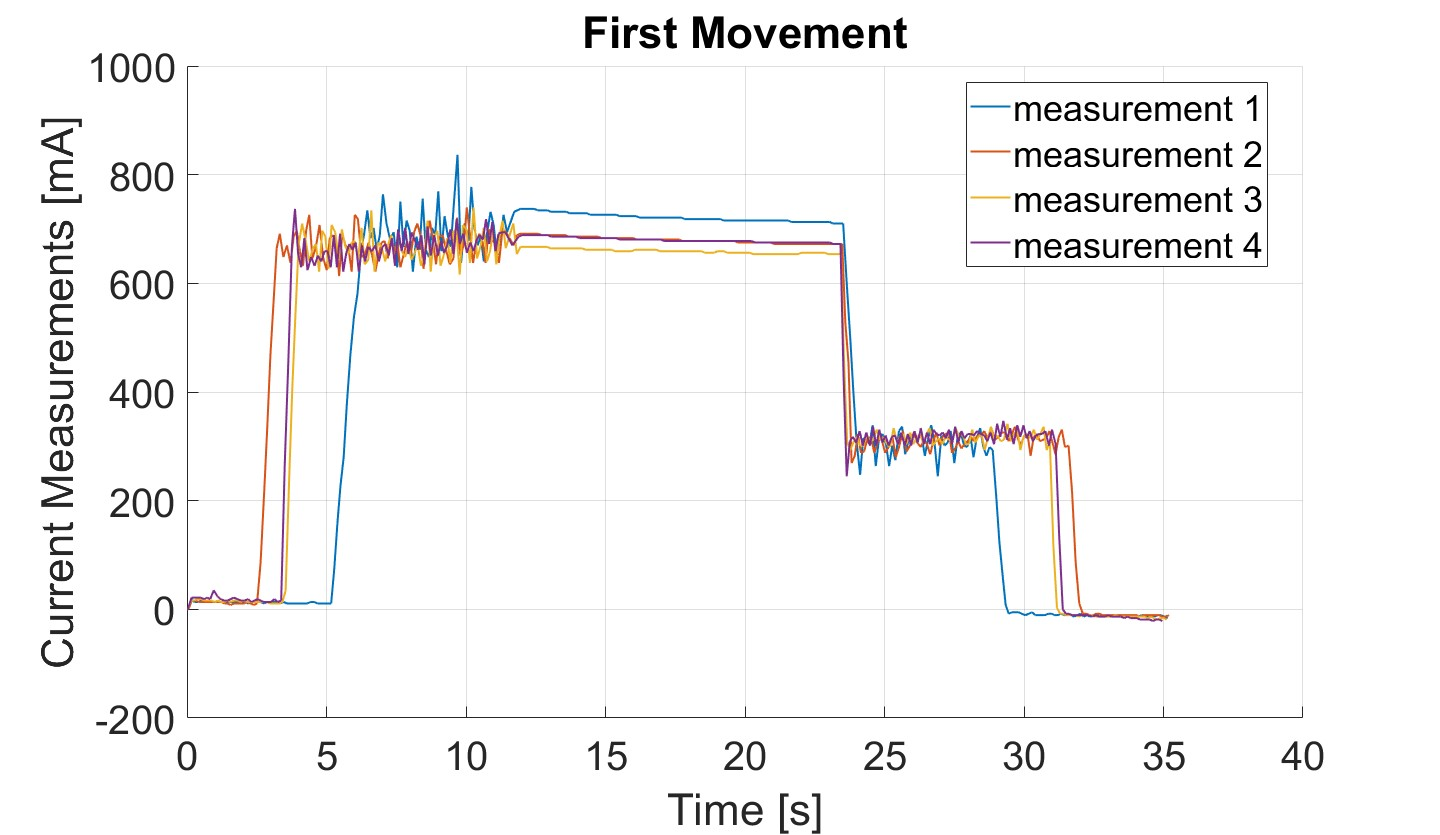
\includegraphics[width=\linewidth]{images/matlab/ex1.jpg}
    \caption{Current measurements for moving an approx. 1 kg weight upwards and downwards.}
    \label{fig:first_measurements}
\end{figure}

As can be seen in the figure, there is a significant difference between the current measurements for hoisting the weight upwards and lowering it downwards.
Each measurement has a slightly different starting time for the upward movement, which is due to the fact that the wheight starts on the ground and the string is initially slack,
therefore the motor needs to wind up some string before the weight starts moving.
It can also be noted that during movement (e.g. from 5s to 10s in \autoref{fig:first_measurements}), the current measurements are a bit noisy,
while when the weight is held in place (e.g. from 12s to 22s in \autoref{fig:first_measurements}), the current measurements are much more stable.
One possible explanation for the difference between the upwards and downwards movement is to assume that there is some internal friction in the motor,
which causes a higher current draw when the motor is working against the external torque.
However it is interesting to note that the current draw when holding the weight in place is equal to the current draw when hoisting the weight upwards,
at least in the experiments so far.
To further investigate this, the weight is lifted by hand, temporarily reducing the applied torque, while the motor is holding the weight in place.
The results of this experiment can be seen in \autoref{fig:holding_weight_upwards}.
\begin{figure}[htbp]
    \centering
    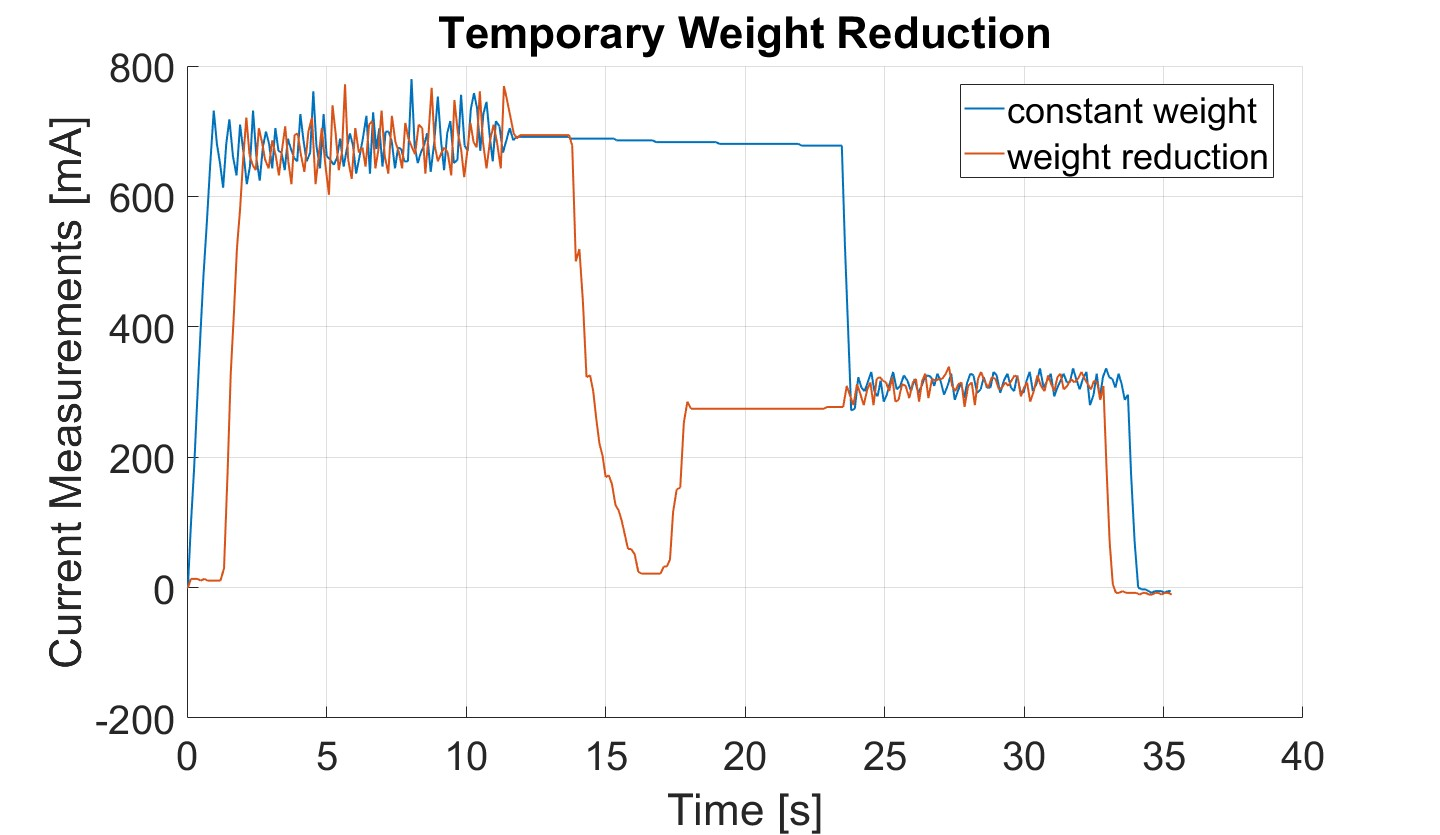
\includegraphics[width=\linewidth]{images/matlab/ex2.jpg}
    \caption{Current measurements when temporarily reducing the applied torque by lifting the weight by hand.}
    \label{fig:holding_weight_upwards}
\end{figure}

By the 20 second mark, the full weight is already being held in place by the motor again, but the current draw has not increased to the previous value.
This experiment shows, that the current measurements when holding the weight in place are not consistent, but depend on the previous movement.
When the weight is lifted by hand, the current draw decreases, as expected, but when the weight is let go again, the current draw increases again to a lower value than before,
equal to the current draw when lowering the weight.
This means that it is not possible to determine one single current-torque relation for static measurements. It also strengthens the assumption that there is some internal friction in the motor,
since the current draw when holding the weight in place after lowering it is lower than when holding it in place after hoisting it upwards.

\subsection{Validating Assumptions}
There are a couple of assumptions that need to be validated before proceeding with further experiments.
\begin{itemize}
    \item First, it needs to be ensured that all four motors behave similarly, so that the results of experiments with one motor can be generalized to all four motors.
    \item Second, it needs to be validated that the measured current is only dependent on the applied torque, and not on other forces, mainly radial loads on the motor axis.
    \item Third, it needs to be validated that the motor behaves similarly for all control modes: position control, current control and velocity control.
\end{itemize}

To validate the first assumption, all four motors were tested one after another with the same movement profile and weight.
The movement profile was slightly modified from the previous experiments to include static phases after both upwards and downwards movement: 
The weight is first lifted, then held in place, then lowered halfway, held again, and finally lowered all the way down.
The results of this experiment can be seen in \autoref{fig:motor_comparison}.
\begin{figure}[htbp]
    \centering
    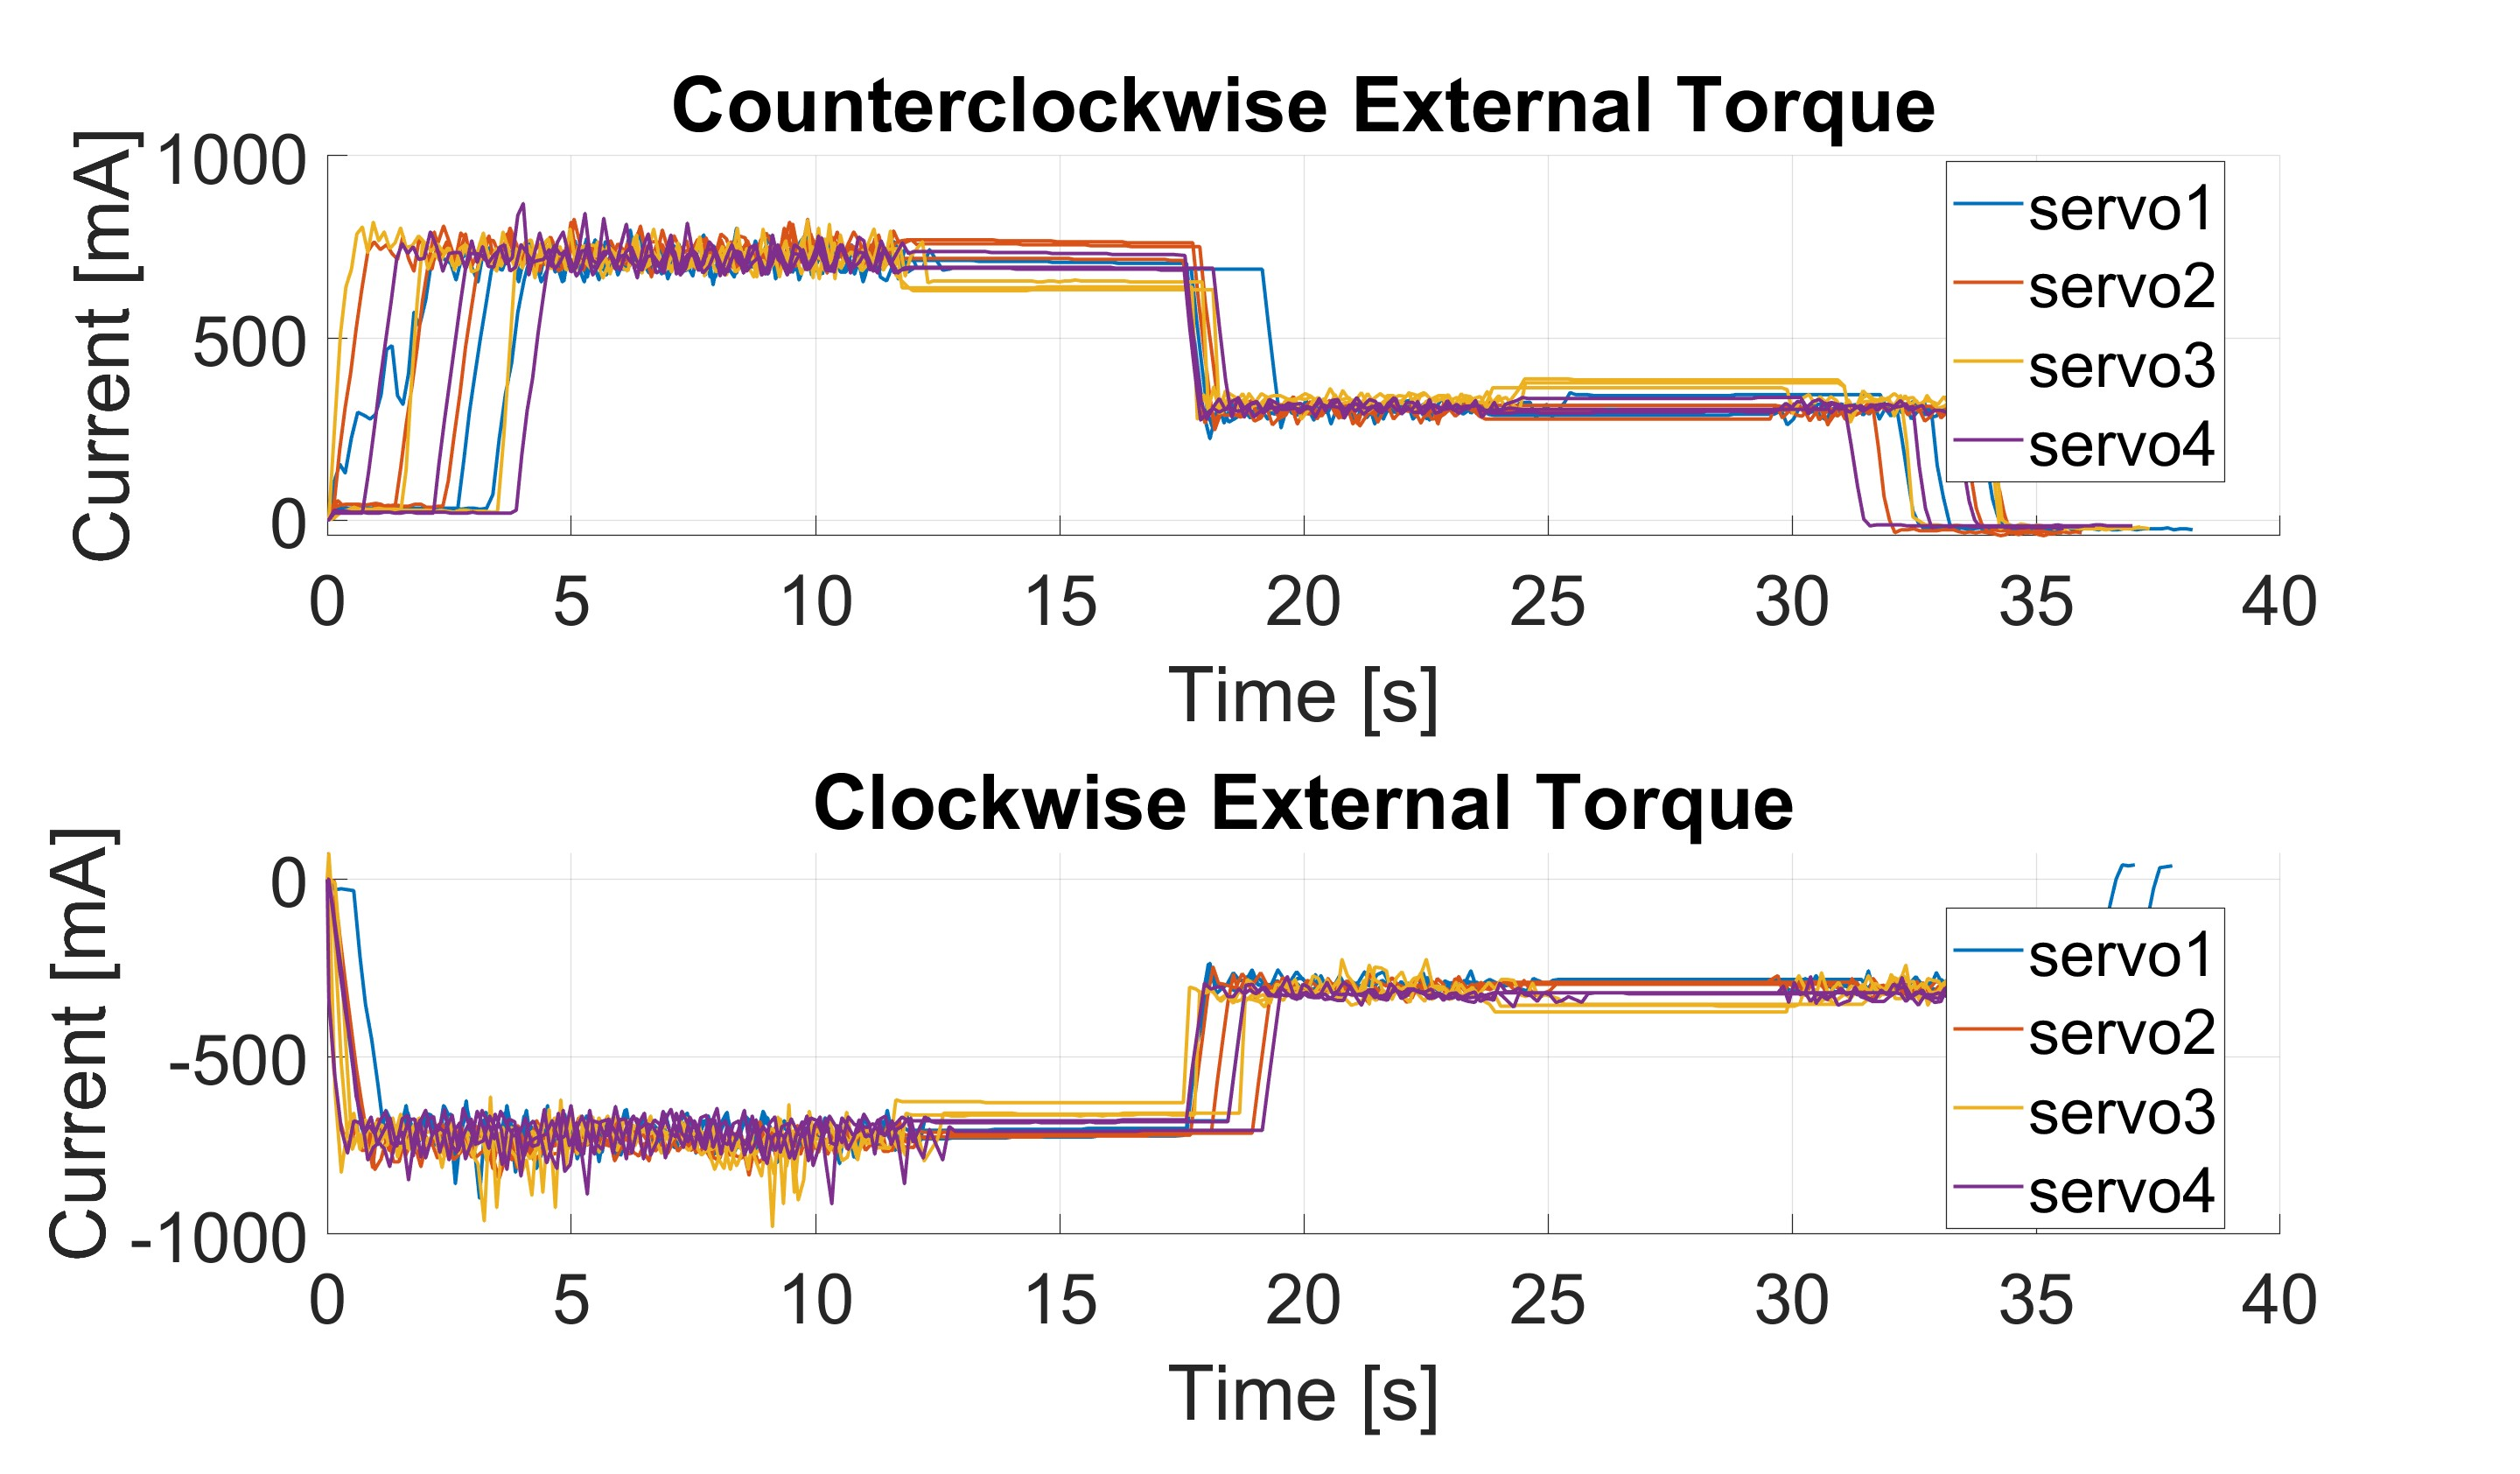
\includegraphics[width=\linewidth]{images/matlab/motor_comparison.jpg}
    \caption{Current measurements for all four motors with a 1 kg weight.}
    \label{fig:motor_comparison}
\end{figure}

As can be seen in the figure, all four motors behave very similarly, validating the assumption that they are interchangeable.
Thus only one motor was used for the following experiments.
Furthermore, the behavior for both directions of applied torque (clockwise and anticlockwise) is also very similar,
validating the assumption that the motor behaves similarly for both directions of applied torque.
Therefore, only one direction of applied torque was used for validating the remaining assumptions.

To validate the second assumption, the string was tied around the axis such that a radial load is applied to the motor axis, instead of a torque.
The motor was then moved in both directions, with and without the radial load. The results of this experiment can be seen in \autoref{fig:radial_load}.
\begin{figure}[htbp]
    \centering
    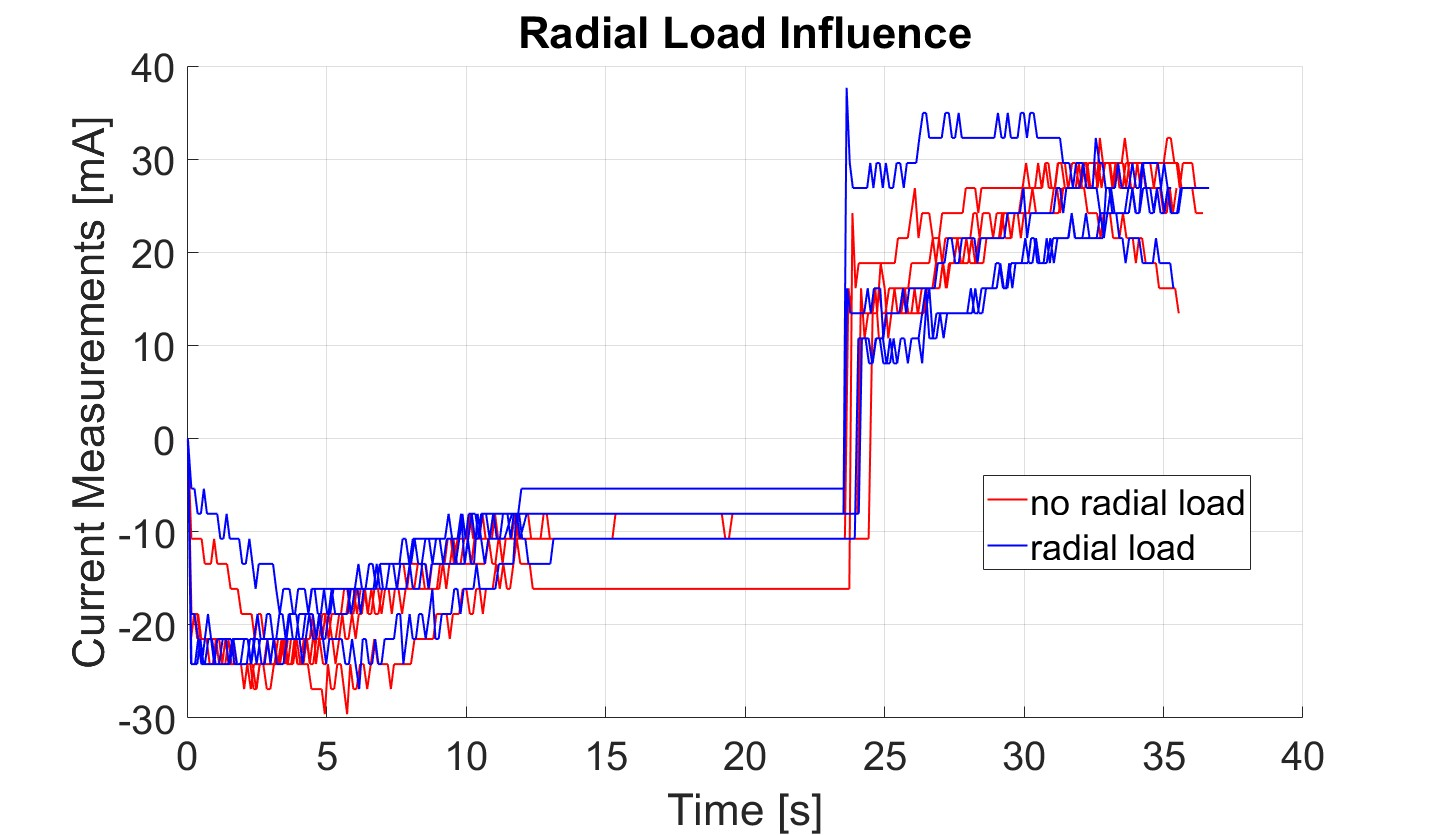
\includegraphics[width=\linewidth]{images/matlab/ex3.jpg}
    \caption{Current measurements with and without radial load on the motor axis.}
    \label{fig:radial_load}
\end{figure}

As can be seen in the figure, there is no significant difference between the current measurements with and without radial load,
validating the assumption that the measured current is only dependent on the applied torque.
It can also be seen that the measurements are very low (max 40mA) compared to the previous experiments (up to 700mA),
which is expected since the motor is not working against any external torque.

To validate the third assumption, two more experiments were conducted, one with position control and one with current control.
The current control experiment was conducted using the same movement profile as before, and can therefore be easily compared to the previous velocity control experiments.
As can be seen in \autoref{fig:current_control}, the results are very similar to the previous velocity control experiments,
validating the assumption that the motor behaves similarly for both control modes.
\begin{figure}[htbp]
    \centering
    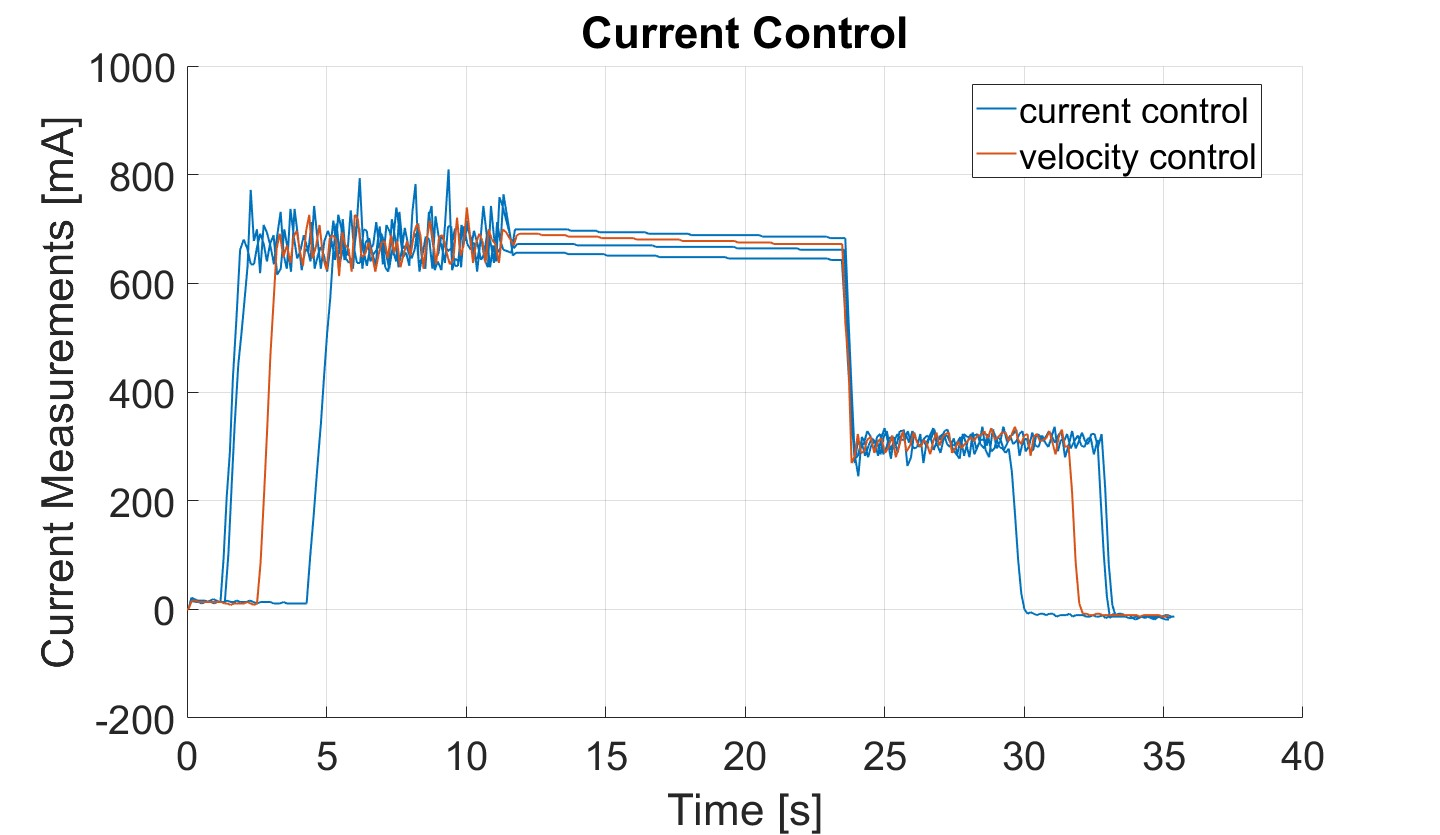
\includegraphics[width=\linewidth]{images/matlab/ex4.jpg}
    \caption{Current Control}
    \label{fig:current_control}
\end{figure}

The position control experiment was conducted by moving the motor to a set position and holding it there for a short moment.
This experiment was also used to further check the behavior of the measured current when holding a changing weight in place.
Similar to \autoref{fig:holding_weight_upwards}, the weight was lifted by hand while the motor was holding it in place.
The results of this experiment can be seen in \autoref{fig:position_control}.
\begin{figure}[htbp]
    \centering
    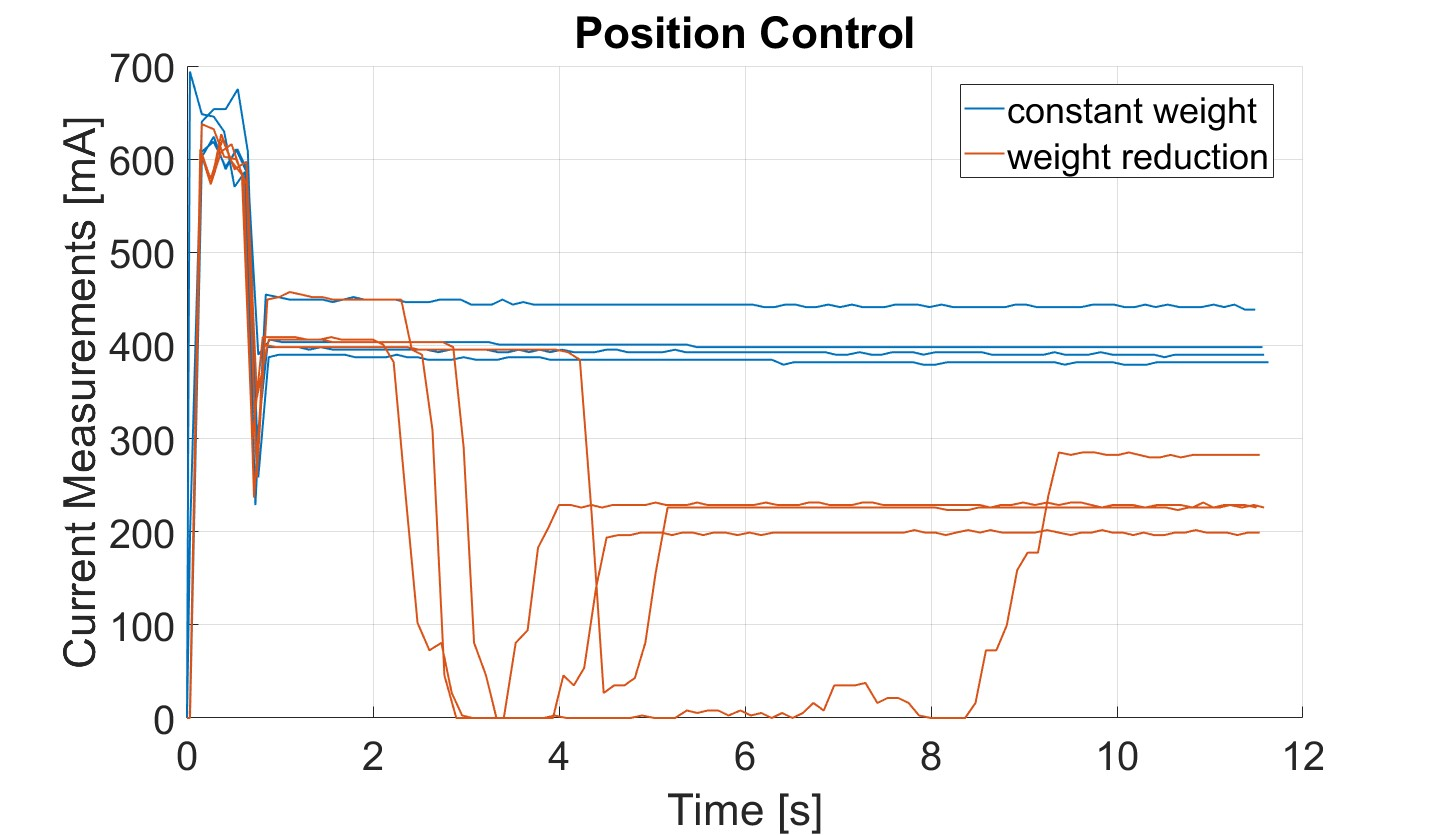
\includegraphics[width=\linewidth]{images/matlab/ex5.jpg}
    \caption{Position Control}
    \label{fig:position_control}
\end{figure}

As can be seen in the figure, the results while the motor is moving are very similar to the previous experiments,
validating the assumption that the motor behaves similarly for position control as well, at least during movement.
The results while holding the weight in place without changing it land somewhere in the 400mA region, which is different than the previous experiments.
Without changing the weight manually, the current for holding the weight in place was either around 700mA (after hoisting upwards) or around 300mA (after lowering downwards).
Similarly to the experiment shown in \autoref{fig:holding_weight_upwards}, the current necessary for holding the 1 kg weight decreases once it has been lifted by hand.
This leads to the conclusion, that while the motor is not moving, the applied torque can not be consistently determined from the measured current,
at least not with the information available from the servo alone.

For future works, the behavior of measurements while the motor is not moving could be further investigated.
One possible approach could be to use a model of the gear resistance and previous movements to better approximate the conversion factor necessary to determine the applied torque
from the measured current. Another approach could be to use an external torque sensor to directly measure the applied torque,
which would evade the problem of gearbox friction.


\subsection{Determining Conversion Factors}
This work will focus on the behavior of the motor while it is moving, where the applied torque can be consistently determined from the measured current.
The goal is to determine the conversion factors from current to torque for both cases: working against applied torque and working with applied torque.

To determine these conversion factors, a new movement profile is used. The weight is only moved dynamically, without any static holding phases.
The weight is first hoisted upwards for the entire distance, then lowered downwards for half the distance, hoisted upwards again for half the distance,
and finally lowered downwards for the entire distance back to the starting position.

For the first experiment, this new movement profile was executed for both directions of applied torque (clockwise and anticlockwise).
The absolute results are gathered and averaged for the two cases (hoisting and lowering weight), as can be seen in \autoref{fig:determine_constant_1Nm}.

\begin{figure}[htbp]
    \centering
    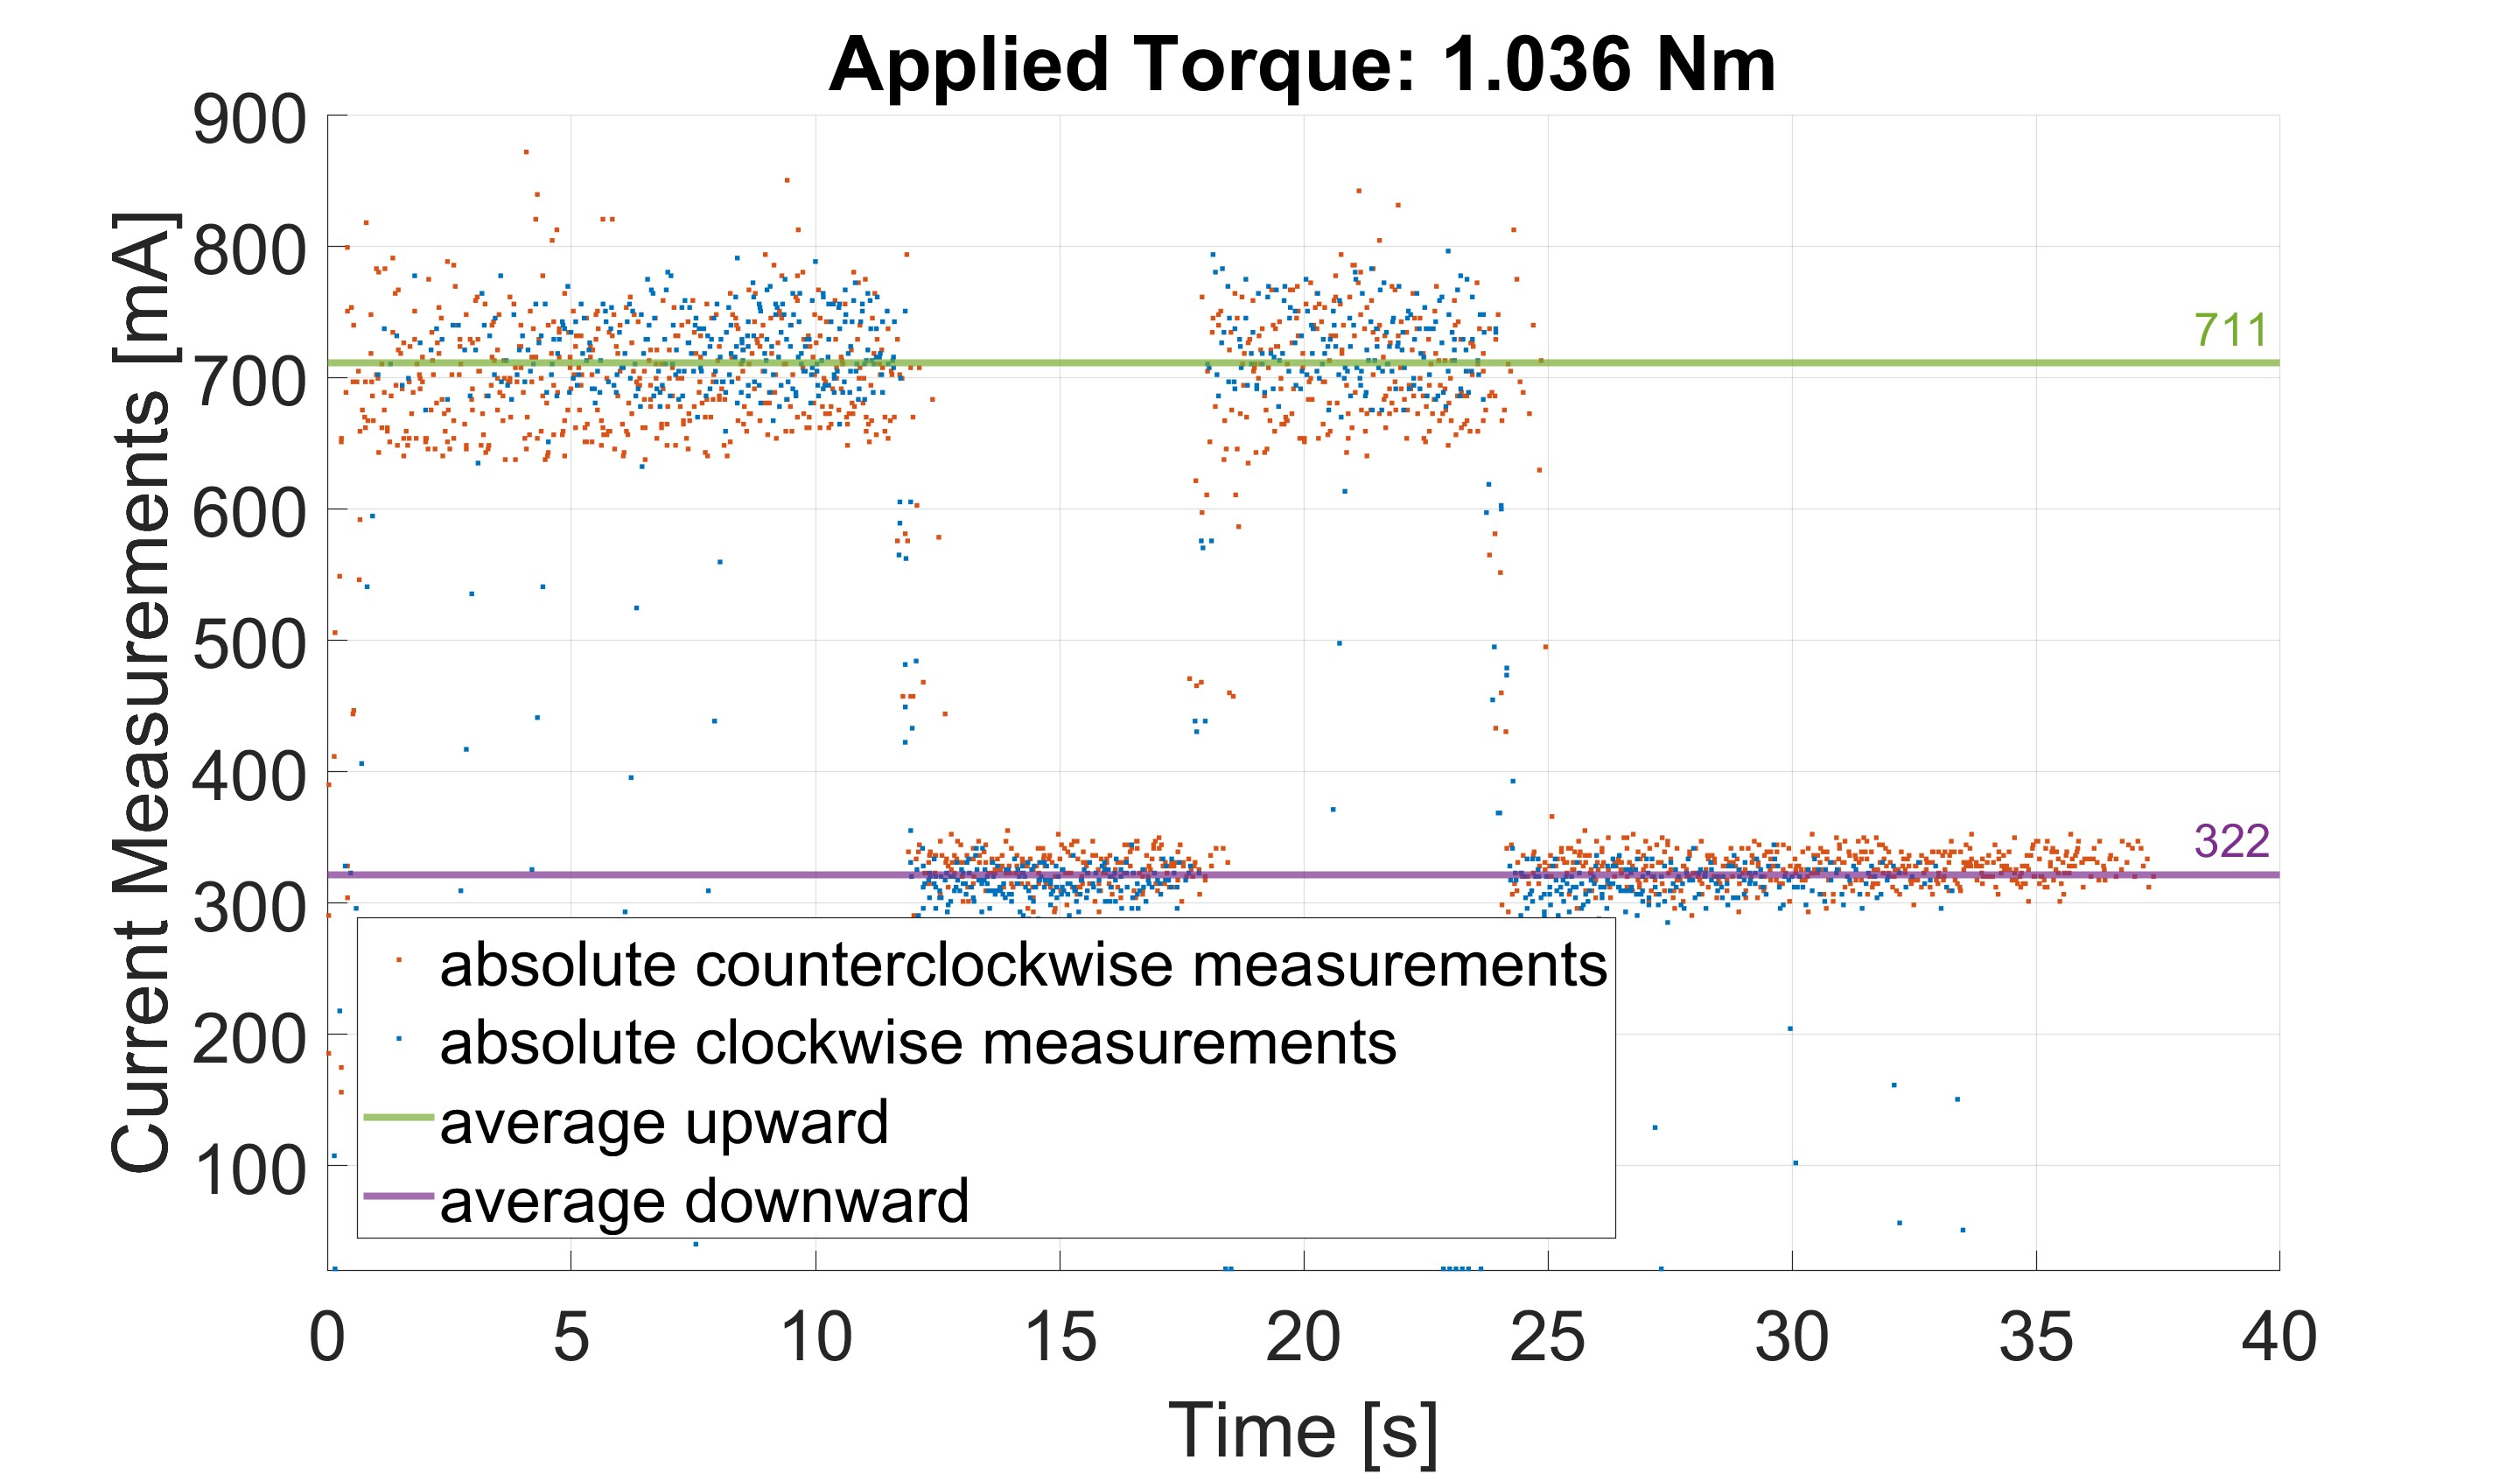
\includegraphics[width=\linewidth]{images/matlab/determine_constant_1Nm.jpg}
    \caption{Current measurements determining the average current draw for working against applied torque (moving upwards) and working with applied torque (moving downwards).}
    \label{fig:determine_constant_1Nm}
\end{figure}
From this experiment, the average current draw for both cases could be determined and thus the conversion factor from current to torque can be computed.
However, since the experiment was only conducted with a 1 kg weight, it cannot be guaranteed that the relation is linear.
Therefore, a second experiment was conducted, where the same movement profile was executed with different weights ranging from 100g to 1 kg.
The measurements taken from this experiment are plotted torque vs current draw, as shown in \autoref{fig:determine_constants_all_weights}.

\begin{figure}[htbp]
    \centering
    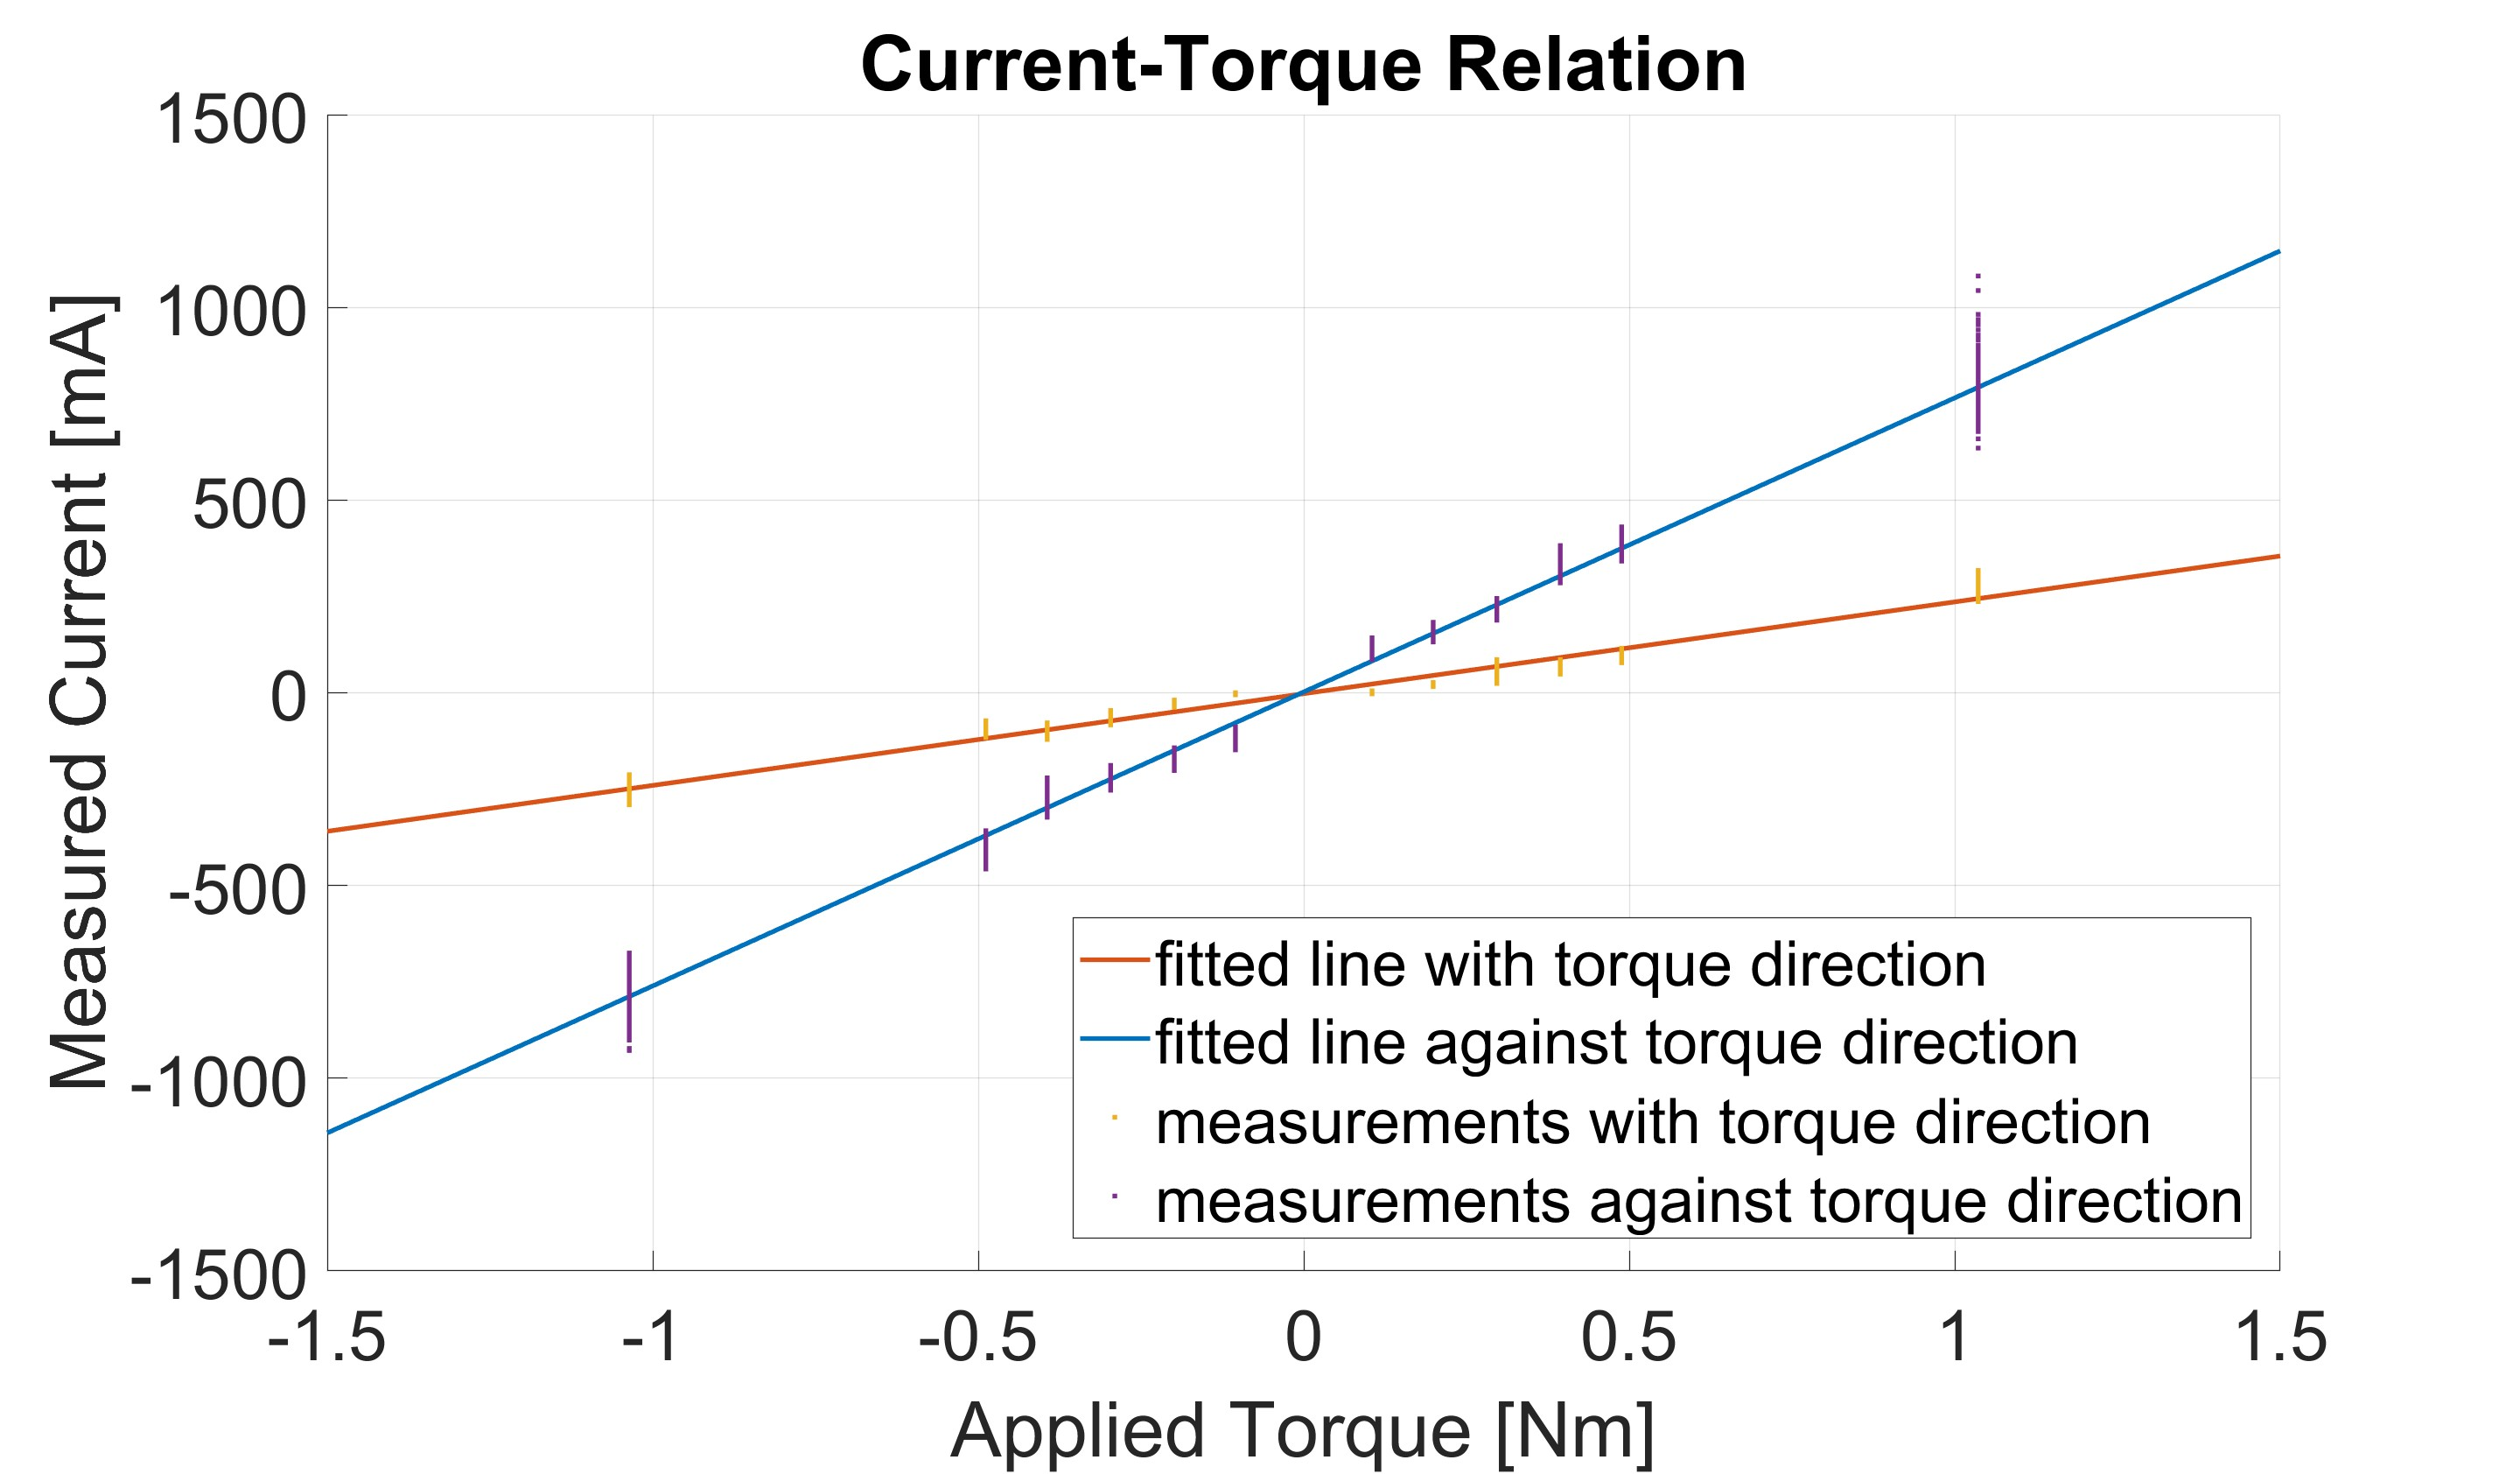
\includegraphics[width=\linewidth]{images/matlab/determine_constants_all_weights.jpg}
    \caption{Current measurements for different weights, determining the relation between applied torque and current draw.}
    \label{fig:determine_constants_all_weights}
\end{figure}
The results show a clear difference between the two cases of working against applied torque (hoisting upwards) and working with applied torque (lowering downwards).
This can be explained by the internal friction of the motor and gearbox: when working against the applied torque, the motor needs to overcome both the external torque and the
internal friction, resulting in a higher current draw for the same applied torque. Similarly, when working with the applied torque, the internal friction reduces the necessary
current draw. This behavior is taken into account by determining two separate conversion factors.
For the two cases it is clear that the relation between applied torque and current draw is linear, therefore they can be modeled with two linear factors:
\begin{itemize}
    \item Working against applied torque (hoisting upwards): $m_{resisiting} = 762.8 \frac{A}{Nm}$
    \item Working with applied torque (lowering downwards): $m_{assisting} = 238.1 \frac{A}{Nm}$
\end{itemize}
Since all static torque measurements measured a current value somewhere between these two factors, it is safe to assume that the conversion factor for the static case,
while not being constant, lies somewhere between these two factors.
\begin{itemize}
    \item Static case (holding weight in place): $m_{resting} \in [238.1, 762.8] \frac{A}{Nm}$
\end{itemize}

\subsection{Implementation}
A set of functions was implemented to read the torque applied to a motor, using the conversion factors determined previously.
In the modular sense of the existing code\parencite{zeitlerDualArmAerialManipulation}, functions were added to read the current and calculate the torque of each servo.
Using the signs of the motors velocity and current measurements to determine the direction of the applied torque, it is decided which conversion factor to use.
For the static case (motor velocity = 0), the function uses the upper limit resting factor, since this is the more conservative choice.

Another function was added which uses the gear ratios of each joint to convert the torque applied to the motor axis into the torque applied to the joint axis.

Finally, a program was written which uses the Jacobian to compute the cartesian force at the end-effector based on
the joint torques using the following formula\parencite{lynchModernRoboticsMechanics2017}:
\begin{equation}
    F = (J^T)^+\,\tau
\end{equation}
Where $\tau$ is the vector of joint torques, $(J^T)^+$ is the pseudoinverse of the transposed Jacobian matrix and $F$ is the vector of cartesian forces at the end-effector.
%\todoZ{cite MR-v2 paper chapter 5}

